\clearpage
\section{Step 4: Design Quality Analysis}
    When talking about the quality of the design of a software, there are a number of aspects that need to be taken into consideration. A well designed software is maintainable, has as few design smells as possible and is, preferably, bug free.\\
    In order to analyse the design quality of the project that we selected, we need to look at certain characteristics, such as the coupling between the components (how tightly or loosely coupled they are), cohesion, what design smells are present, why, and how they can be mediated. In the following sections, we will document our findings about the design quality of OptaPlanner.\\
    To help us with the analysis, we will use all the previously acquired knowledge about the system (from steps 2 and 3), and at the same time, we will also use a new tool called Designite 
    \footnote{Designite home page: \url{http://www.designite-tools.com/}}.
    
    \subsection{Designite}
        According to the official documentation:\\
        \begin{adjustwidth}{1.5cm}{}
            \textit{Designite is a software design quality assessment tool. It analyzes code
            and identifies software quality issues. Specifically, it detects a comprehensive set 
            of architecture, design, and implementation smells and provides mechanisms such as detailed metrics analysis, 
            Dependency Structure Matrix, trend analysis, and smell distribution maps.}
        \end{adjustwidth}
        \vspace{0.5cm}
        From the official description, we can conclude that this tool can help us with the design quality analysis of our chosen OSS. The tool seems to be focusing on the types of metrics that we are interested in, and the architecture analysis that it provides can help us better understand OptaPlanner. \\
        For the purpose of this document, we have used the \texttt{DesigniteJava Community Edition} 
        \footnote{DesigniteJava CE: \url{https://www.designite-tools.com/designitejava/community}}.
        The official documentation provides us with a list of all the smells that Designite can detect. We will not list them here, but the smells will be mentioned and explained when they are encountered in OptaPlanner.\\
        
    \subsection{Method of analysis}
        Using Designite to analyse a project is rather simple and straight-forward. From the official website we have downloaded a \texttt{jar} file, which we can then use to run on the path where the code of the project is found. To do so, we have used the following command:
        \begin{lstlisting}
java -jar DesigniteJava.jar -i optaplanner -o designite-output   \end{lstlisting}
        The \cb{-i} and \cb{-o} flags are used to denote the input and output folders respectively. \\
        After running the tool, the output of the analysis can be found in the \cb{designite-output} folder. The following files have been generated:
        \begin{itemize}
            \item \texttt{designCodeSmells.csv}
            \item \texttt{implementationCodeSmells.csv}
            \item \texttt{methodMetrics.csv}
            \item \texttt{typeMetrics.csv}
        \end{itemize}
        \textbf{Note:}
            \begin{adjustwidth}{1cm}{}
            We will make use of the information found in these files to analyze the design quality of the project. The results, together with all the numbers, occurrences of the smells and their locations can be traced back to these files.
            \end{adjustwidth}
        \clearpage
        
\section*{Results}
    In this section, we will discuss the results of our analysis on the design quality of the OptaPlanner system. We will discuss the following aspects:
    \begin{enumerate}
        \item The \textbf{cohesion} of the system
        \item The degree of \textbf{coupling} between the components
        \item The \textbf{design and architectural smells} found in the system
        \item The most 'smelly' components wrt. both code and design smells
    \end{enumerate} 
    Each topic will be analysed and argued for, together with examples and representative graphs.
    
    \subsection{Cohesion}
        By definition, \textit{cohesion refers to the degree to which the elements inside a module belong together}
        \footnote{Cohesion definition: \cb{\url{https://en.wikipedia.org/wiki/Cohesion\_(computer\_science)}}}.
        The advantages of having a highly cohesive system are multifold:
        \begin{itemize}
            \item Modules have reduced complexity (due to the fact that they are simpler and have fewer operations)
            
            \item It helps when following the Single-Responsibility Principle (SRP) of entities having responsibility over a single functionality 
            
            \item The system becomes more maintainable, since changes in the domain will affect a lower number of components, and as such, less components need to be modified. As such, it helps with the prevention of the Shotgun-Surgery code smell (making modifications requires many small changes to many different classes).
            \footnote{Shotgun-Survey smell:  \cb{\url{https://refactoring.guru/smells/shotgun-surgery}}}
            
            \item It increases the system's reusability, since components can be easily reused if a module has a highly cohesive set of operations
        \end{itemize}
                
        \subsubsection{LCOM}
            In order to detect how cohesive a system is, the code has to be analysed at a very granular level, and the cohesion of each class can be computed. In order to calculate cohesion, a certain metric can be used: \textbf{LCOM}. It stands for Lack of Cohesion in Methods, and it is a measure for the number of not conected pairs in a class representing independent parts having no cohesion. LCOM represents the difference between the number of methods not having instance variables in common, and the number of methods having common instance variables
            \footnote{A more detailed overview of LCOM:
            \cb{\url{http://www.arisa.se/compendium/node116.html}}}. \\
            When talking about the value of LCOM, a low value is desirable and it indicates a highly/totally cohesive class. A high value indicates low cohesion. This makes sense, since a low "lack of cohesion" score implies a lot of cohesion.\\\\
            Designite can compute the LCOM metrics in its' analysis. The values of LCOM are between 0 and 1, 0 indicating strong cohesion and 1 indicating total lack of cohesion. \\\\
            \textbf{Note:}
            \begin{adjustwidth}{1cm}{}
            The analysis can also return the value \texttt{-1} for LCOM - and according to the developers
            \footnote{Negative LCOM value: \cb{\url{https://github.com/tushartushar/DesigniteJava/issues/66}}}
            this value is used to indicate that LCOM could not be computed for this certain class/file because information was missing or LCOM was not applicable (eg. due to the file being an interface or abstract).\\
            \end{adjustwidth}
            \textbf{LCOM threshold value}\\
            By looking at the documentation, we have found that Designite also has the ability to set a certain threshold for a metric, meaning that whenever this threshold is reached or surpassed, the tool will mark it as a metric violation. In the case of LCOM, the threshold value is 0.8. In our analysis, we will also use LCOM = 0.8 as the treshold value for marking 'bad' classes. 
            
        \subsubsection{Cohesion metrics}
            According to Designite, the \cb{optaplanner-core} has 38 classes whose LCOM value is higher than the threshold, indicating a low cohesion and potential candidate classes for refactoring. 
            Taking into considerating that this is a project of substantial size, and that the algorithms implemented are not trivial, such a small number of classes with low cohesion is a very good one and it shows the the system is highly maintainable. Moreover, we could also say that the system has, overal, high cohesion, and we can safely asume that the developers kept this aspect in mind at all times while writing the code. 
            \begin{figure}[H]
                \centering
                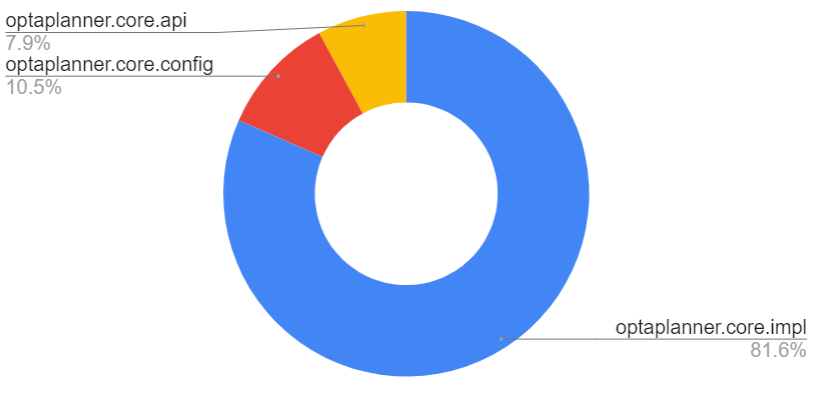
\includegraphics[scale=0.6]{figures/step4/corelowcohesion.PNG}
                \caption{Distribution of low cohesion classes in the \cb{optaplanner-core} folder}
                \label{fig:corelowcohesion}
            \end{figure}
            As we knew from the previous steps that inside the \cb{core} package, the \cb{impl} folder is the biggest and most complex, we also expected this folder to contain the most classes with low cohesion. The analysis confirms this, since designite found that out of the 38 classes, 32 were found in the \cb{impl} folder. An overview of the number of classes in each of the three folders can be seen in Figure \ref{fig:corelowcohesion}. 
            \\\\
            In order to see which particular locations inside the most complex folder contain the most problematic classes, we analysed the \cb{impl} folder at a lower level and we have found that there are two locations which contain a high number of such classes. Figure \ref{fig:lowcohesion} depicts the overall distribution of the classes in the \cb{impl} folder. 
            \begin{figure}[H]
                \centering
                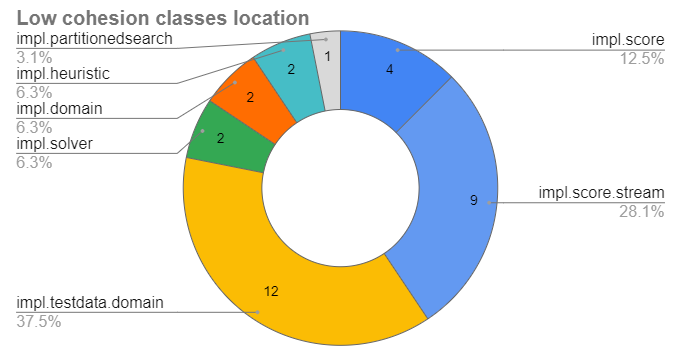
\includegraphics[scale=.7]{figures/step4/lowcohesion.PNG}
                \caption{Distribution of classes with a high LCOM score value in the \cb{optaplanner-core/impl} folder}
                \label{fig:lowcohesion}
            \end{figure}
            From this figure, we can see that the two locations \cb{impl.score} and \cb{impl.testdata.domain} contain the most classes that have a low cohesion (13 and 12 respectively) and should therefore be the first candidates to refactor, in order to increase the cohesion of the system. Inside these two folders, there were 8 classes whose LCOM score was 1 - meaning that they are totally non-cohesive, and that are difficult to maintain and they also add to the technical debt of the project. Outside these two locations, there were 3 other classes with an LCOM score of 1. The classes can be found at the following locations:              
            \begin{itemize}
                \item \cb{org.optaplanner.core.impl.partitionedsearch.TestdataFaultyEntity.java}
                \item \cb{org.optaplanner.core.impl.domain.common.accessor.MemberAccessorFactory.java}
                \item \cb{org.optaplanner.core.impl.solver.thread.ThreadUtils.java}
            \end{itemize}
            In the development life cycle, every time a new feature is introduced or changed, risk is being introduced. If the new feature requires the developer to look all around the code base to implement changes, the risk increases. At the same time, if classes have incoherent and unrelated functionalities piled up together, the risk of breaking the code or introducing bugs becomes close to inevitable when the new feature should be added.\\
            LCOM can be seen as a metric that warns developers of the parts of the code that are becoming risky, and it can help prevent bugs rather than solving them. At the same time, it can also warn of a design that is not entirely optimal. These concerns are very important for the development of clean, maintainable code, and as such, LCOM can definitely be of assistance for a project. \\
    \subsection{Coupling between components}
            According to the definition
            \footnote{Coupling definition: \cb{
            \url{https://en.wikipedia.org/wiki/Coupling\_(computer\_programming)}}}:
            \begin{adjustwidth}{1.5cm}{}
                \textit{coupling is the degree of interdependence between software modules; a measure of how closely connected two routines or modules are; the strength of the relationships between modules.}
            \end{adjustwidth}
            Tight coupling in a software system can be associated with more interdependency between components, more coordination and more information flow; on the other hand, low coupling can be associated with less interdependency, coordination and information flow. \\
            Tightly coupled systems can have the following characteristics, often seen as disadvantages:
            \begin{enumerate}
                \item A change in one module can cause a ripple effect of changes in other modules 
                \item Assembly of modules will take considerably longer time thanks to the increased interdependency between them and the high flow of information
                \item Using a single module as a standalone might be difficult due to other modules also being needed.
            \end{enumerate}
            Looking at these characteristics, we can motivate the general idea that good design usually is related to loose coupling in the system.\\\\
            In order to analyze the design quality of the system, we have to analyze the coupling between its components. As such, we will make use of two metrics, namely \texttt{FANIN} and \texttt{FANOUT}. These two metrics were borrowed from logic circuit design, and they represent the number of occurrences of a class (how many times a class is being called) and the number of classes a certain class calls in its definition. They can be used to indicate the extent to which a component is independent, as well as how much responsibility is has.\\
            When describing packages, we can talk about two types of coupling:
            \begin{enumerate}
                \item \textbf{Afferent coupling AC}\\
                The number of packages that depend upon classes in a certain package. It indicates the package's responsibility.
                \item \textbf{Efferent coupling EC}\\
                The number of packages that the classes in a package depend upon. It indicates the package's independence.
            \end{enumerate}
            
    \subsection{Design and architectural smells}
        By definition, 
        \begin{adjustwidth}{1.5cm}{}
            \textit{design smells are structures in the design that indicate violation of the fundamental design principles and negatively impact design quality}\footnote{Design Smells definition: \cb{\url{https://en.wikipedia.org/wiki/Design_smell}}}.
        \end{adjustwidth}
        Design smells indicated the accumulated design debt, which is one of the most important dimensions of technical debt. Bugs are not seen as design smells - instead, they arise from the poor design decisions that make the design unstable and difficult to maintain.\\\\
        Using the Designite tool, we should be able to find 17 design smells in our code. However, not all of those were present in the project. In the following sections, we will take a look at each of the three components individually and explore the present design smells. \\
        Afterwards, the most common smells will be discussed, together with possible remedies.\\\\
        
        \begin{itemize}
            \item \textbf{The \cb{api} folder}\\
            There are currently 133 design code smells in this folder. The most frequent one is \cb{Unutilized Abstraction}, appearing 66 times. The second most frequent smell is \cb{Insuficient Modularization}, appearing 30 times, and the third \cb{Unnecessary Abstraction}, 17 times. Figure \ref{fig:apidesignsmells} gives an overview of all of the smells in this folder.
            \begin{figure}[H]
                \centering
                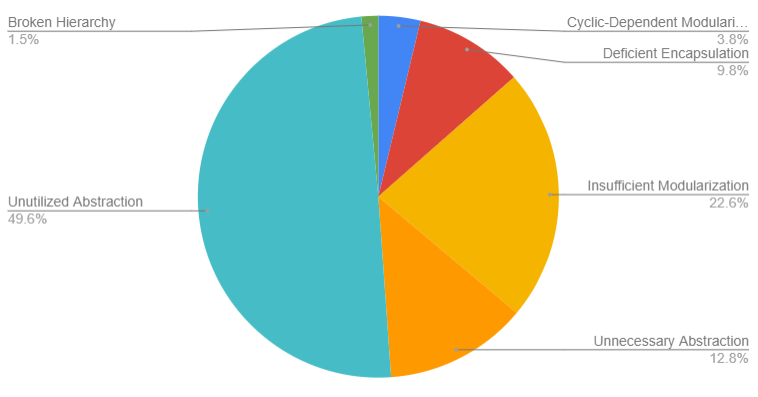
\includegraphics[scale=0.7]{figures/step4/designsmellapiPNG.PNG}
                \caption{Design smells found in the \cb{api} folder and their frequency}
                \label{fig:apidesignsmells}
            \end{figure}
            In this folder, there was no file that stood out with a high number of smells. The files had at most two smells, usually being \cb{Unutilized Abstraction} paired up with one of the others.
            
            \item \textbf{The \cb{config} folder}\\
            This folder has the least amount of design smells, summing up to 49. Out of those, the most frequent ones are: \\
            \cb{Unitilized Abstraction, Insuficient Modularization, Deficient Encapsulation} appearing 24,23 and 6 time respectively. Figure \ref{fig:configdesignsmells} gives an overview of all the smells in this folder.
             \begin{figure}[H]
                \centering
                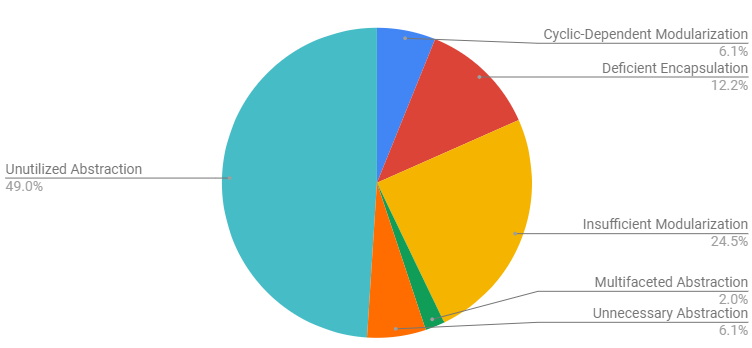
\includegraphics[scale=.8]{figures/step4/designsmellconfig.PNG}
                \caption{Design smells found in the \cb{config} folder and their frequency}
                \label{fig:configdesignsmells}
            \end{figure}
            While most of the files in this folder also had at most two design smells, the file\\ 
            \cb{org.optaplanner.core.config.solver.SolverConfig.java} has three, namely: \\
            \cb{Cyclic-Dependent Modularization, Deficient Encapsulation, Insufficient Modularization}; perhaps this class could be a good starting point for refactoring in order to improve the cohesion of the project.
            
            \item \textbf{The \cb{impl} folder}\\
            Again, since this folder is the biggest and most complex, it is not a surprise that the most design smells are situated here. In total, the tool has found 861 design smells, out of which the most occurring one is \cb{Unutilized Abstraction}, appearing 521 times. The second one, \cb{Cyclic-Dependent Modularization} appears 166 times and the third most occurring is \cb{Broken Hierarchy}, 83 times. Figure \ref{fig:impldesignsmells} gives a better overview of all the design smells that appear in this package, together with their names and frequencies.
            \begin{figure}[H]
                \centering
                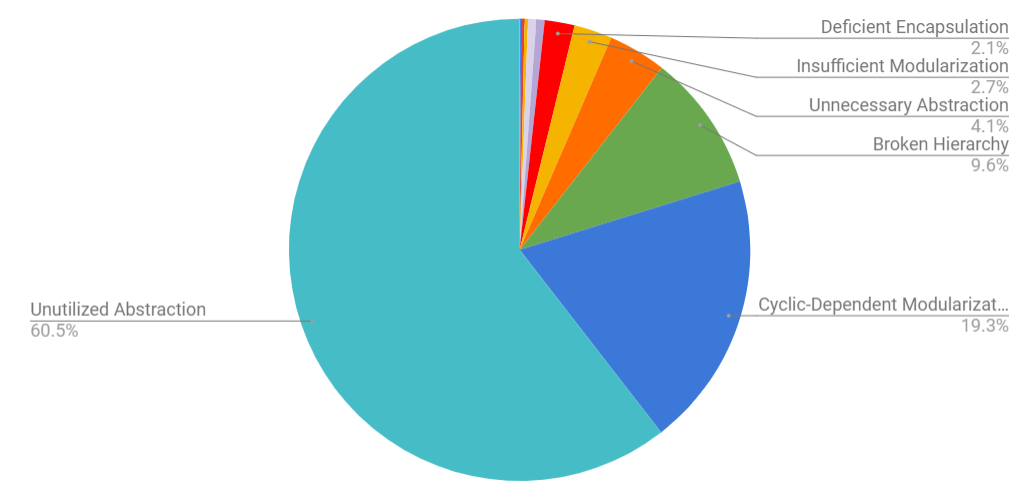
\includegraphics[scale=0.7]{figures/step4/designsmellimpl.PNG}
                \caption{Design smells found in the \cb{impl} folder and their frequency}
                \label{fig:impldesignsmells}
            \end{figure}
            When looking inside this folder for the file with the most design smells, we have found that the following files\\ 
            \cb{org.optaplanner.core.impl.domain.entity.descriptor.EntityDescriptor.java} and \\
            \cb{org.optaplanner.core.impl.domain.solution.descriptor.SolutionDescriptor.java} have 3 design smells: \\
            \cb{Cyclic-Dependent Modularization, Deficient Encapsulation, Insufficient Modularization}. This is the same combination of three smells that we have encountered in the previous package as well. It could be that they are closely related, and that the presence of one could increase the chances of the other being present. 
        \end{itemize}
        
        \subsubsection{Code smells analysis}
        \begin{itemize}
            \item From the previous section, we can deduce that the most occurring design smell is \cb{Unutilized Abstraction}. It is the most occurring smell in every folder, appearing a total of 611 times in the whole \cb{optaplanner-core} package. This smell arises when an abstraction is left unused, either not directly or not reachable. The unused abstraction does not play any role in the functionality, thus violating the abstract principle. Unrealized abstract classes and interfaces are superfluous and could be seen as imaginary summaries, so they are not needed and might be confusing as to why they are there in the first place. \\
            There can be a couple of reasons why this design smell might occur.
            \begin{itemize}
                \item It could be that the developer wanted to design a 'timeless' solution for a  problem, with the thought that it might be useful in the future. 
                \item Another reason could be that the initial requirements changed, and the abstraction to solve the initial problem was no longer needed, but was still left in the design.
                \item It could also be caused by developers failing to clean up old code when maintaining or refactoring, leaving the abstraction unreferenced and leading to the design smell.
                \item Lastly, it could be that the developers did not remove the abstraction due to uncertainty about whether it is used somewhere else or not.
            \end{itemize}
            The best way to deal with this smell is by removing the abstraction from the design. APIs that might be used by external parties without the developer's knowledge could be marked as Obsolete and the new clients should be informed not to make use of them any more.
            
            \item Another commonly occurring smell is \cb{Insufficient Modularization}. This smell appears when the abstraction has not been completely decomposed, and a further decomposition could reduce its size, implementation complexity, or both. This could be as a result of classes growing over time, being assigned more functionalities and responsibilities, and the developers failing to see that together with this the cohesion of the class decreases. It could also be that this abstraction is being used by multiple different clients, however, having one single file accommodate all of the requirements of the clients can be troublesome and lead to reduced extensibility and changeability.\\
            This smell breaks the design rule: \textit{Decompose abstractions to manageable size.}\\\\
            To solve this problem, the best solution would be to split up the abstraction into smaller abstractions that are more cohesive and have the smallest size and complexity possible.
            
            \item \cb{Cyclic Dependency Modularization} is another design smell that is commonly occurring. Cyclic dependencies appear when two or more abstractions depend on each other. When this happens, the abstractions need to be understood, used, tested and modified together, and changes on one of them might have to be reflected into the others. \\ 
            This smell breaks the design rule:
            \textit{Create acyclic dependencies.} \\
            A reason why this smell could occur is that the members of one abstractions are misplaced in a different abstraction, making the first one depend on the second and thus resulting in a cyclic dependency. Another reason could be that a class passes a self reference in a method call (for example, using \texttt{doSomething(this)}. \\\\
            The way to solve this design smell is by breaking the dependency cycle. One possible solution could be to introduce an interface for one of the abstractions in the cycle. Another possible solution would be to move the code that introduces the dependency to a different abstraction. Or, if possible, to merge the abstractions that are cyclically dependent into a single one.
        \end{itemize}
 